% Adjust these for the path of the theme and its graphics, relative to this file
%\usepackage{beamerthemeFalmouthGamesAcademy}
\usepackage{../../beamerthemeFalmouthGamesAcademy}
\usepackage{multimedia}
\graphicspath{ {../../} }

% Default language for code listings
\lstset{language=C++,
        morekeywords={each,in,nullptr}
}

% For strikethrough effect
\usepackage[normalem]{ulem}
\usepackage{wasysym}
\usepackage{gensymb}
\usepackage{pdfpages}

% http://www.texample.net/tikz/examples/state-machine/
\usetikzlibrary{arrows,automata}

\newcommand{\modulecode}{COMP260}\newcommand{\moduletitle}{Distributed Systems}\newcommand{\sessionnumber}{5}

\begin{document}
\title{\sessionnumber: Session title here}
\subtitle{\modulecode: \moduletitle}

\frame{\titlepage} 

\begin{frame}
	\frametitle{Immersion}
	Immersion is the objective degree to which a VR system and application projects stimuli onto the sensory receptors. 

	\begin{itemize}
		\item Extensiven
		\item Matching
		\item Surrounding
		\item Vividness
		\item Interactability
		\item Plot
	\end{itemize}
\end{frame}

\begin{frame}
	\frametitle{Perceptual Modalities}
	
	Sight, hearing, touch, proprioception, balance/motion, smell and taste. 
		
\end{frame}

\begin{frame}
	\begin{figure}
		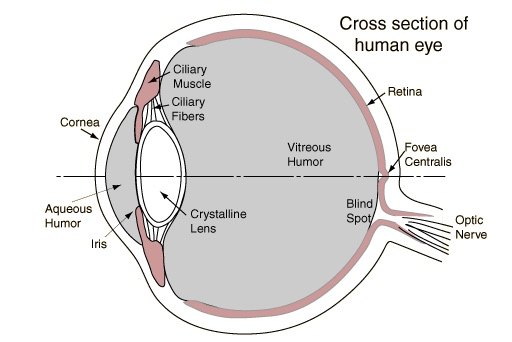
\includegraphics[scale=.6]{assets/eye} 
		\caption{}
	\end{figure}
\end{frame}


\begin{frame}
	\frametitle{Cones and Rods}
	\begin{figure}
		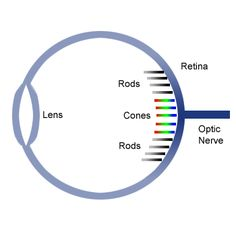
\includegraphics[scale=.5]{assets/cones-rods.jpg}
		\caption{ The retina is covered in two types of photoreceptors, cones and rods. Cones are responsible for vision in ideal conditions and rods are responsible for low light levels and non-ideal conditions. }
	\end{figure}
\end{frame}


\begin{frame}
	\frametitle{Central vs. Peripheral Vision}
	\textbf{Central}
	\begin{itemize}
		\item has high visual acuity,
		\item optimised for bright daytime conditions, and
		\item is color sensitive.
	\end{itemize}
	
	\textbf{Peripheral Vision}
	\begin{itemize}
		\item is color insensitive, 
		\item is more sensitive to light than central vision in dark conditions,
		\item is less sensitive to longer wavelengths (i.e., red),
		\item has faster response and has more sensitive to fast motion and flicker, and
		\item is less sensitive to slow motions.
	\end{itemize}
\end{frame}

\begin{frame}
	\frametitle{Field of View and Field of Regard}
	%The \textbf{field of view} is the angular measure of what can be seen at a single point in time. 
	\begin{figure}
		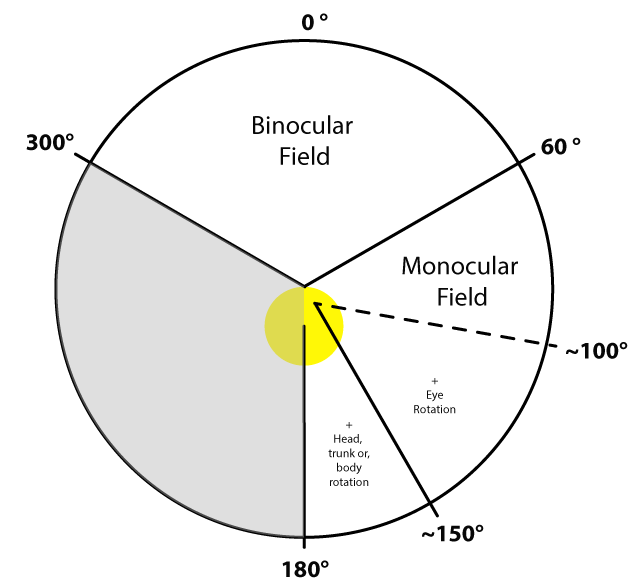
\includegraphics[scale=.3]{assets/fov} 
		\caption{Horizontal field of view of the right eye with straight ahead fixation (looking towards the top of the diagram)}
	\end{figure}
\end{frame}

\begin{frame}
	\frametitle{Visual Pathways}

\end{frame}

\begin{frame}
	\frametitle{acuity}
	Visual Acuity is the ability to resolve details and often measured in visual angle. \\~\\ \pause
	
	A fifty pence coin held at arms length has an angle of acuity of 2\degree \\~\\ \pause
	
	A fifty pence coin held up at 81 meters away has an angle of acuity of 1/60th of a degree. \\~\\ \pause
	
	In perfect conditions a human can see a line as thin as 1/7200th of a degree. 
\end{frame}

\begin{frame}
	\begin{figure}
		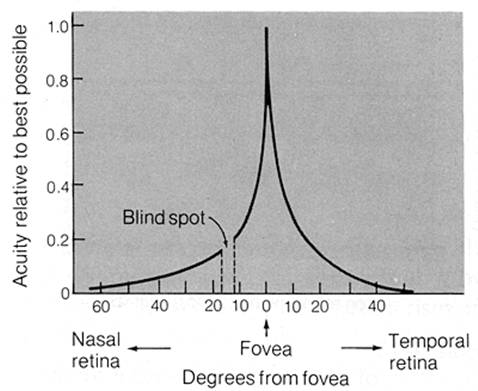
\includegraphics[scale=.9]{assets/acuity} 
		\caption{Visual acuity is much better at the fovea.}
	\end{figure}
\end{frame}

\begin{frame}
The evidence suggests that if you consider that the each eye about 210\degree including rotation and that stereoscopic acuity is
\end{frame}
\begin{frame}
	\frametitle{VR Lenses}
	\begin{center}
		\href{https://www.youtube.com/watch?v=NCBEYaC876A}{ 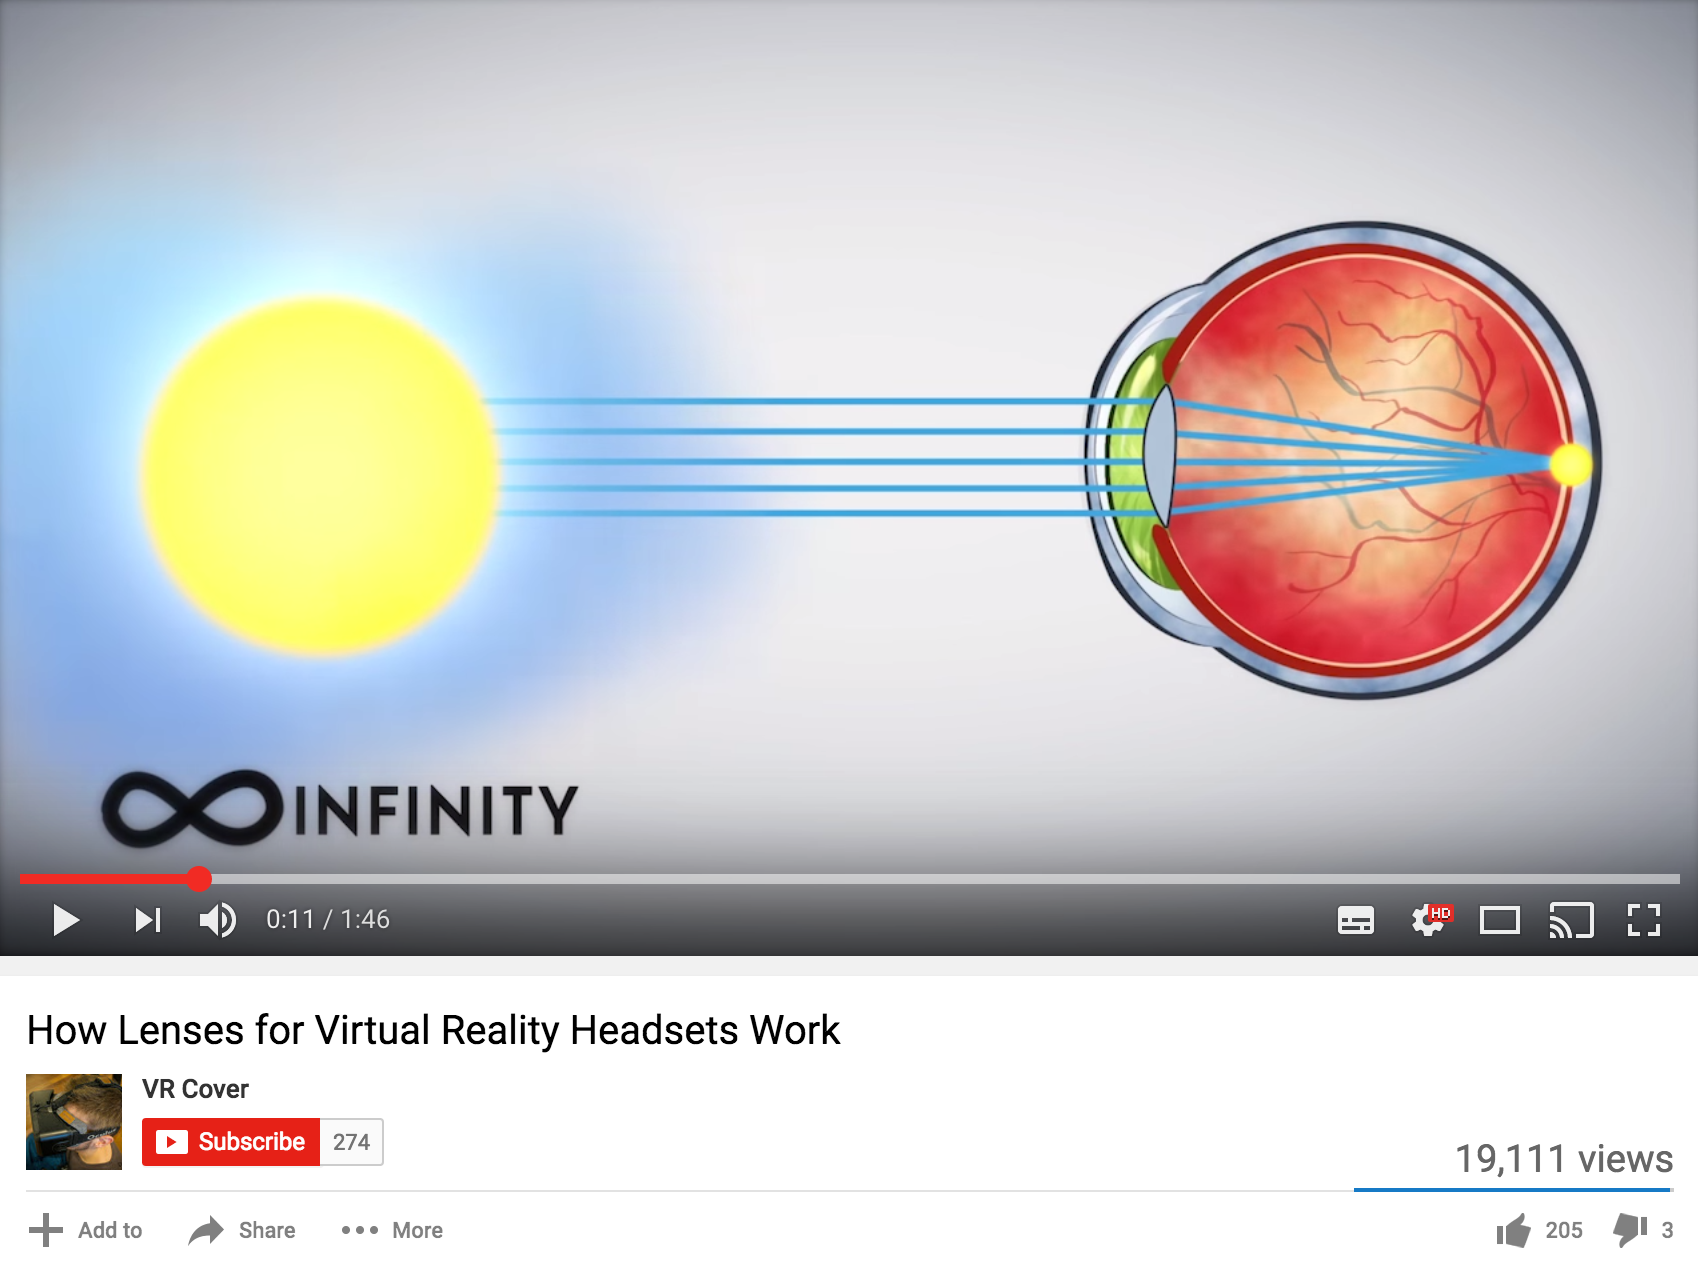
\includegraphics[scale=.3]{assets/lenses}  }
	\end{center}
\end{frame}

\begin{frame}
	\frametitle{Foveated Rendering}
	\begin{center}
		\href{https://www.youtube.com/watch?v=6q3w0fiD0zg}{ 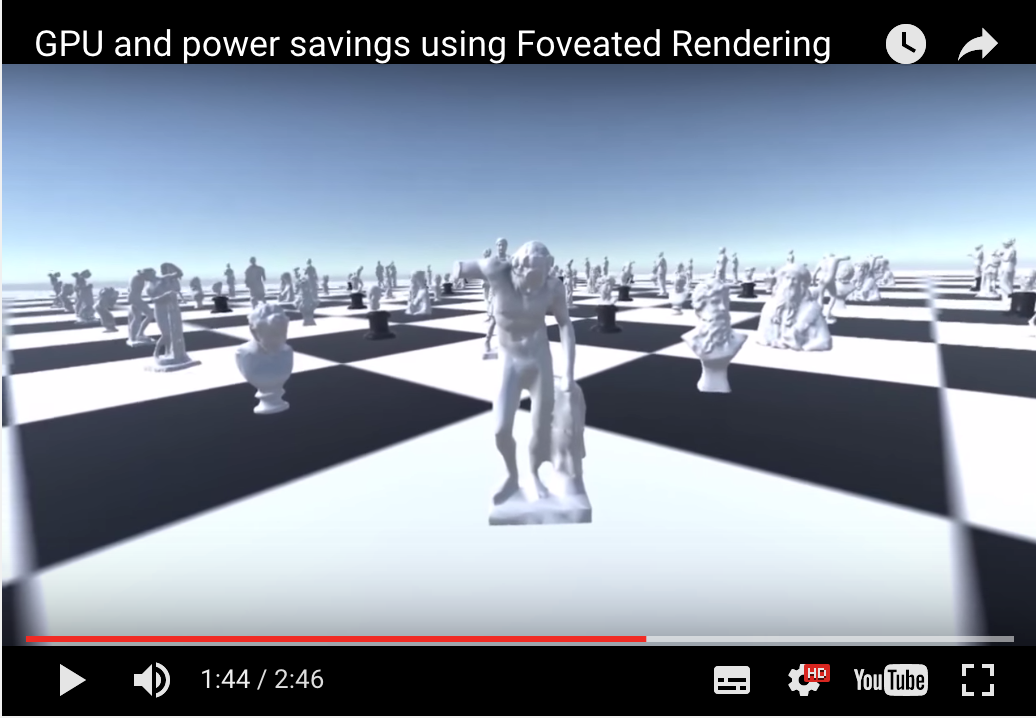
\includegraphics[scale=.4]{assets/foveated-rendering}  }
	\end{center}
\end{frame}

\begin{frame}
	

\end{frame}


\begin{frame}
	\frametitle{Eye Tracking Demo} 
\end{frame}


\end{document}
